\section{The Butterfly Lovers}

\textbf{Matgioi} was one of five Europeans initiated into the Chinese Primordial Tradition. He divided it into three stages, each associated with a teacher, or actually a collective entity. As he put it:

\begin{quotex}
The first of men, \textbf{Fuxi} \emph{crystallized} the Primordial Tradition, \textbf{Lao Tzu} drew from it a body of doctrine, \textbf{Confucius} drew from it a system of morality.

\end{quotex}
The three parts were to appear in three works:

\begin{enumerate}
\item \emph{Metaphysical Path,} the principles of the Tradition and its philosophical and cosmogonic movement. (\emph{I Ching}) 
\item \emph{Rational Path} relates the systematization of Tradition, with Taoism, or \emph{Tao Te Ching} of Lao Tzu 
\item \emph{Social Path} relates the adaptation of the Tradition, with the political philosophy of Confucius (Analects) 
\end{enumerate}
The third volume never appeared.

\paragraph{The Figurists}
The Jesuit missionaries considered the I Ching to be a prophetic book containing the mysteries of Christianity. They also recognized the ancient origins of Chinese civilization, which predated the Flood. Shem, the son of Noah, was thought to have brought the Primordial Tradition from Adam to China.

Moreover, they believed that Fuxi, Zoroaster, Hermes Trismegistus, and the prophet Enoch were the same person. Matgioi mentions none of this.

\paragraph{Fuxi}
Although Fuxi claimed that he drew his teaching from much older sources, he is symbolically recognized as the first human being. Nuwa, his sister and wife, was Eve to his Adam. Together, they are the Androgyne. That is represented in the symbol of the Yin Yang. Matgioi explains the union and separation:

\begin{quotex}
The eternal androgyne separates only to fertilize itself … the father and the mother exist only to create: at the moment of creation, they are united and form only one; at the moment they separate, the seed exists.

\end{quotex}
\paragraph{Birth and Death}
Matgioi explains the process of birth and death:

\begin{quotex}
Man is not free in his birth nor in his death. For his birth, he is free neither of acceptance, nor of refusal, nor of the moment. As for death, he is not free to avoid it … Birth launches him irresistibly onto the \emph{circulus} of an existence which he neither asked for nor chose. Death withdraws him from this \emph{circulus}, and launches him irresistibly into another, prescribed and foreseen by the Will of Heaven.

\end{quotex}

\begin{wrapfigure}{rt}{.35\textwidth}
 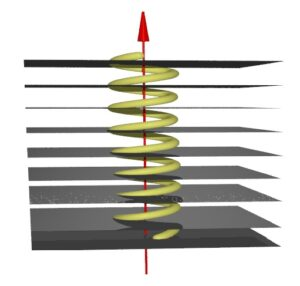
\includegraphics[scale=.5]{a20221002TheButterflyLovers-img001.jpg} 
 \end{wrapfigure}

The Will of Heaven lifts him onto higher and higher stages of life. Matgioi represents this as a series of planes, with a vertical line indicating the Will of Heaven. A helix, centered along the vertical line, illustrates the ascent from plane to plane. Death at one plane is birth at the next. As Matgioi describes it:

\begin{quotex}
death at the end of cycle X is greater than birth on the same cycle X, by the whole value of the attraction of heaven's will upon the cycle X, that is to say mathematically the value of the pitch of the evolutionary helix.

\end{quotex}
Hence, death is nothing to fear

\begin{quotex}
The phenomenon of death is identical, absolutely, and it seems to us to determine analogous effects, but in the opposite direction, only because we have fallen into the bad habit of considering it from the sole point of view of human state. The \emph{exit} from this state (death) corresponds to the dispersion of the body, to the loss of the human material form, which is the lowest part of our compound. But the entry into the suprahuman state (birth) which is coincident with human death, involves the accession of a spiritual element, the value of which we do not know, and which is superior to the best of our human elements. This is why human death, since it coincides with a better birth, is superior, metaphysically, to human birth.

\end{quotex}
\paragraph{Iconography}

The iconography illustrates this. Fuxi and Nuwa are united in Heaven as the Androgyne. Each has as helix that represents their ascents through the planes of existence. They are intertwined indicating that they make that ascent together, as One.

\begin{wrapfigure}{rt}{.2\textwidth}
 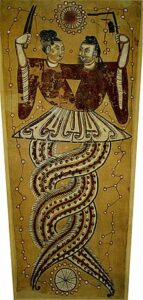
\includegraphics[scale=3]{a20221002TheButterflyLovers-img002.jpg} 
\end{wrapfigure}

\paragraph{The Butterfly Lovers}
Metaphysical teachings are often hidden in popular culture and stories. The story of the Butterfly Lovers\footnote{\url{https://en.wikipedia.org/wiki/Butterfly_Lovers}}, one of China's Four Great Folktales, is an example. Zhu disguises herself as a man to attend classes where she meets Liang. They have an immediate affinity and Zhu falls in love with Liang. Because he believes Zhu is a man, he cannot reciprocate that love in the way she wants.

Eventually, Zhu's father finds a husband for her. She is forced to return home. When Liang visits her later on, she reveals that she is a woman. They express their love to each other. But Zhu must marry another. Liang then dies of a broken heart.

On the wedding procession, Zhu passes Liang's grave. She leaves the procession to visit it. Suddenly the earth opens up and Zhu jumps in. Liang and Zhu then emerge as butterflies, never to separate again.

This shows that what appears to be death is actually birth into a higher degree of existence.

\url{https://www.youtube.com/watch?v=sOuPpyuqcOE}

H/T to Prasad for the helix diagram.



\flrightit{Posted on 2022-10-02 by Cologero }
